\documentclass[CJKutf8,xcolor=pdftex,dvipsnames,table]{beamer}
\usepackage{hyperref}
\hypersetup{
  pdftitle={Operating System Concepts},
  pdfauthor={Hong MingJian},
  pdfsubject={Process Synchronization},
  pdfpagemode={FullScreen},
  colorlinks={true},
  linkcolor={blue},
}
\usepackage{CJKutf8}
\usepackage{listings}
\lstset{
	language=[ANSI]C,
	basicstyle=\scriptsize,
	tabsize=2,
	breaklines=true,
	keywordstyle=\color{blue},
	identifierstyle=,
	commentstyle=\color{OliveGreen},
	stringstyle=,
	showstringspaces=false,
  extendedchars=false
%  numbers=left,
%  numberstyle=\tiny
}

\usetheme{Madrid}%{Warsaw}
\usecolortheme{crane}

%gets rid of bottom navigation bars
\setbeamertemplate{footline}[page number]{}
%gets rid of navigation symbols
\setbeamertemplate{navigation symbols}{}

\begin{document}
\begin{CJK*}{UTF8}{song}

  \title{\CJKfamily{hei} 操作系统原理}
  \subtitle{\CJKfamily{hei} 第七章:进程同步}
  \author{\CJKfamily{hei} 洪明坚}
  \institute{\CJKfamily{hei} 重庆大学软件学院}
  \date{\today}

  \AtBeginSection[]
  {
    \begin{frame}
      \frametitle{Outline}
      \tableofcontents[currentsection]
    \end{frame}
  }

  \frame{\titlepage}

  \frame{\frametitle{目录}\tableofcontents}

\section{Race condition}

  %% PAGE
  \begin{frame}
  \frametitle{Background} \pause
  \begin{itemize}
  \item{Cooperating processes may share a block of memory via IPC facilities provided by the kernel.} \pause
    \begin{itemize}
    \item{Multiple threads within a process may share a piece of memory by using global variables.} \pause
    \end{itemize}
  \item{Concurrent access to shared data may result in data inconsistency.} \pause
    \begin{itemize}
    \item{Maintaining data consistency requires mechanisms to ensure the orderly execution of cooperating processes.} \pause
    \end{itemize}
  \item{Solution to \emph{producer and consumer problem} (Chapter 4) allows at most \textit{(BSIZE - 1)} items in buffer at the same time.} \pause
    \begin{itemize}
    \item{A solution, where all \textit{BSIZE} buffers are used is NOT simple.} \pause
    \item{Suppose that we modify the code by adding a variable \textit{counter}.}
    \end{itemize}
  \end{itemize}
  \end{frame}

  %% PAGE
  \begin{frame}[fragile]
  \frametitle{Producer and consumer problem} \pause
  \begin{itemize}
  \item{Shared-memory bounded-buffer} \pause
  \end{itemize}
\begin{lstlisting}
                   /* Shared variables */
                   #define BSIZE 10
                   struct item {
                      ....
                   } buffer[BSIZE];
                   int in = 0, out = 0, counter = 0;
/*---------------------------------------------------------------*/
/*The producer loop*/                 /*The consumer loop*/
while(1) {                            while(1) {
  /*produce an item*/                   while(counter == 0)
  while(counter == BSIZE)                 /*do nothing*/;
    /*do nothing*/;                     itemConsumed = buffer[out];
  buffer[in] = itemProduced;            out = (out + 1) % BSIZE;
  in = (in + 1) % BSIZE;                counter--;
  counter++;                            /*consume the item*/
}                                     }
\end{lstlisting}
\end{frame}

  %% PAGE
  \begin{frame}[fragile]
  \frametitle{Problem of above solution (1/2)} \pause
  \begin{itemize}
  \item{When producer and consumer processes are executed \emph{concurrently}, they may not function correctly.} \pause
    \begin{itemize}
    \item{We can show that the value of \textit{counter} may be incorrect as follows.} \pause
    \end{itemize}
  \item{Note that the ``\textit{counter}$++$'' and ``\textit{counter}$--$'' may be implemented in machine language as} \pause
  \end{itemize}

\begin{lstlisting}
        ; counter++
        register1 = counter        ; load the counter to a register
        register1 = register1 + 1  ; add
        counter = register1        ; write back

        ; counter--
        register2 = counter        ; load the counter to a register
        register2 = register2 - 1  ; subtract
        counter = register2        ; write back
\end{lstlisting}

\end{frame}

  %% PAGE
  \begin{frame}
  \frametitle{Problem of above solution (2/2)} \pause
  \begin{itemize}
  \item{It's important to note that the above two instruction sequences can be \emph{interleaved} because of interrupts or scheduling.} \pause
  \item{For example, assume \textit{counter} is initially 5,} \pause
  \end{itemize}
  \rowcolors[]{1}{blue!20}{blue!10}
  \begin{tabular}{c|c|c|c}
    Time & Producer                & Consumer              & result\\
    \hline \pause
    $T_0$   & register1=\textit{counter}       &                       & \{register1=5\}\\ \pause
    $T_1$   & register1=register1+1   &                       & \{register1=6\}\\ \pause
    $T_2$   &                         & register2=counter     & \{register2=5\}\\ \pause
    $T_3$   &                         & register2=register2-1 & \{register2=4\}\\ \pause
    $T_4$   & \textit{counter}=register1       &                       & \{\textit{counter}=6\}\\   \pause
    $T_5$   &  & \textit{counter}=register2     & \{\textit{counter}=\color{red}4\color{black}\}     \pause
  \end{tabular}
  \begin{itemize}
  \item{The value of \textit{counter} may be either 4 or 6, while the correct result should be 5.}
  \end{itemize}
  \end{frame}

  %% PAGE
  \begin{frame}
  \frametitle{Questions}
  \begin{itemize}
  \item{Any questions?}
  \end{itemize}
  \begin{center}
    
\includegraphics[scale=.5]{question}
  \end{center}
  \end{frame}

  %% PAGE
  \begin{frame}
  \frametitle{Race condition (1/2)} \pause
  \begin{itemize}
  \item{\emph{Race condition is a situation where several processes access and manipulate the same data concurrently and the outcome of the execution depends on the particular order in which the access takes place}.} \pause
  \item{How do we avoid race condition?} \pause
    \begin{itemize}
    \item{Find some way to prohibit more than one process from reading and writing the shared data concurrently.} \pause
    \item{That is, the access must be \emph{serialized} even if the processes attempt concurrent access.}
    \end{itemize}
  \end{itemize}
  \end{frame}

  %% PAGE
  \begin{frame}
  \frametitle{Race condition (2/2)} \pause
  \begin{itemize}
  \item{\textbf{Critical section}} \pause
    \begin{itemize}
    \item{a piece of code where the shared resource is accessed.} \pause
    \end{itemize}
  \item{A solution of race condition must satisfy the following 4 requirements:} \pause
    \begin{enumerate}
    \item{\textbf{Mutual exclusion}: No two process may be simultaneously inside their critical section;} \pause
    \item{\textbf{Progress}: No process running outside its critical section may block other processes trying to enter its critical section;} \pause
    \item{\textbf{Bounded waiting}: No process should have to wait forever to enter its critical section;} \pause
    \item{\textbf{Speed}: No assumptions may be made about speeds or the number of the CPUs.}
    \end{enumerate}
  \end{itemize}
  \end{frame}

  %% PAGE
  \begin{frame}[fragile]
  \frametitle{Critical section} \pause
  \begin{itemize}
  \item{A protocol must be designed to be used by the processes to enter and leave critical section.} \pause
    \begin{itemize}
    \item{Each process must request permission to enter its critical section.} \pause
    \end{itemize}
  \end{itemize}

\begin{lstlisting}
                        do {
                          <entry section>

                          CRITICAL SECTION

                          <exit section>

                        } while (1);
\end{lstlisting}

  \pause

  \begin{itemize}
  \item{In the following slides, we will try to construct several ``entry
    section'' and ``exit section'' to solve the race condition.}
  \end{itemize}
\end{frame}

  %% PAGE
  \begin{frame}
  \frametitle{Questions}
  \begin{itemize}
  \item{Any questions?}
  \end{itemize}
  \begin{center}
    
\includegraphics[scale=.5]{question}
  \end{center}
  \end{frame}

\section{Possible solutions to race condition}

\subsection{Software solutions}

  %% PAGE
  \begin{frame}[fragile]
  \frametitle{First try} \pause
  \begin{itemize}
  \item{Assume there are only two cooperating processes: $P_i$ and $P_j$, where i+j=1.} \pause
  \end{itemize}

\begin{lstlisting}
                   int turn = 0; // or 1
                   do {
                     while(turn != i);  // entry section

                     CRITICAL SECTION

                     turn = j;          // exit section

                   } while (1);
\end{lstlisting}

  \begin{itemize}
  \item{Does it satisfy all 4 requirements for a solution?} \pause
    \begin{itemize}
    \item{No, it breaks the \textbf{progress} requirement.}
    \end{itemize}
  \end{itemize}
\end{frame}

  %% PAGE
  \begin{frame}[fragile]
  \frametitle{Second try} \pause

\begin{lstlisting}
                   bool flag[2] = {false, false};
                   do {
                     // entry section
                     flag[i] = true;
                     while(flag[j]);

                     CRITICAL SECTION

                     flag[i] = false; // exit section

                   } while (1);
\end{lstlisting}

  \begin{itemize}
  \item{Does it satisfy all 4 requirements for a solution?} \pause
    \begin{itemize}
    \item{No, it breaks the \textbf{progress} requirement too.}
    \end{itemize}
  \end{itemize}
\end{frame}

  %% PAGE
  \begin{frame}[fragile]
  \frametitle{Third try} \pause

\begin{lstlisting}
                   int turn = 0; // or 1
                   bool flag[2] = {false, false};
                   do {
                     // entry section
                     flag[i] = true;
                     turn = j;
                     while(flag[j] && turn == j);

                     CRITICAL SECTION

                     flag[i] = false; // exit section

                   } while (1);
\end{lstlisting}

  \begin{itemize}
  \item{Does it satisfy all 4 requirements for a solution?} \pause
    \begin{itemize}
    \item{Yes, it's a correct solution and is known as \emph{Peterson's algorithm}.}
    \end{itemize}
  \end{itemize}
\end{frame}

  %% PAGE
  \begin{frame}[fragile]
  \frametitle{Bakery algorithm} \pause
  \begin{itemize}
  \item{Peterson's algorithm solves the problem for two processes, while \emph{Bakery algorithm} solves it for multiple processes.} \pause
  \end{itemize}

\begin{lstlisting}
          bool choosing[n] = {false, ..., false};
          int number[n] = {0, ..., 0};
          do {
            // entry section
            choosing[i] = true;
            number[i] = max(number[0], ..., number[n-1])+1;
            choosing[i] = false;
            for(j=0; j < n; j++) {
              while(choosing[j]);
              while((number[j]!=0)&&(number[j],j)<(number[i],i));
            }

            CRITICAL SECTION

            number[i] = 0; // exit section

          } while (1);
\end{lstlisting}

\end{frame}

  %% PAGE
  \begin{frame}
  \frametitle{Questions}
  \begin{itemize}
  \item{Any questions?}
  \end{itemize}
  \begin{center}
    
\includegraphics[scale=.5]{question}
  \end{center}
  \end{frame}

\subsection{Hardware solutions}

  %% PAGE
  \begin{frame}
  \frametitle{Synchronization hardware} \pause
  \begin{itemize}
  \item{Several low-level hardware features may be used to solve the race condition.} \pause
    \begin{enumerate}
    \item{Disabling interrupts} \pause
    \item{Special instructions} \pause
      \begin{itemize}
      \item{TSL (Test and Set Lock)} \pause
      \item{SWAP}
      \end{itemize}
    \end{enumerate}
  \end{itemize}
  \end{frame}

  %% PAGE
  \begin{frame}
  \frametitle{Disabling interrupts} \pause
  \begin{itemize}
  \item{The CPU is only switched from process to process as a result of clock or other interrupts.} \pause
    \begin{itemize}
    \item{Once a process has disabled interrupts, it can access the shared memory without fear that any other process will intervene.} \pause
    \end{itemize}
  \item{Example - INTEL x86} \pause
    \begin{itemize}
	\item{CLI (\textbf{cl}ear \textbf{i}nterrupt) - turn off interrupt} \pause
	\item{STI (\textbf{s}e\textbf{t} - \textbf{i}nterrupt) turn on interrupt} \pause
    \end{itemize}
  \item{Disadvantages} \pause
    \begin{enumerate}
    \item{User processes should NOT be able to disable the interrupts;} \pause
      \begin{itemize}
	  \item{CLI/STI are both privileged instructions} \pause
	  \end{itemize}
    \item{It's not feasible in a multiprocessor system.}
    \end{enumerate}
  \end{itemize}
  \end{frame}

  %% PAGE
  \begin{frame}[fragile]
  \frametitle{TSL and SWAP (1/3)} \pause
  \begin{itemize}
  \item{The TSL and SWAP instructions have the following functionalities, respectively:} \pause
  \end{itemize}

\begin{lstlisting}
						bool TSL(bool &target)     void SWAP(bool &a, bool &b)
						{                          {
						  bool rv = target;          bool temp = a;
						  target = true;             a = b;
						  return rv;                 b= temp;
						}                          }
\end{lstlisting}

  \pause

  \begin{itemize}
  \item{Bear in mind that TSL and SWAP are executed \emph{atomically}, that is, as one uninterruptible unit.}
  \end{itemize}
\end{frame}

  %% PAGE
  \begin{frame}[fragile]
  \frametitle{TSL and SWAP (2/3)} \pause
  \begin{itemize}
  \item{Use TSL or SWAP to TRY to solve race condition} \pause
  \end{itemize}

\begin{lstlisting}
						  bool lock = false;               bool lock=false;
						  do {                             do {
						    // entry section                 // entry section
						    while(TSL(lock))                 bool key = true;
						      ;                              while(key == true)
						                                       SWAP(lock, key);

						    CRITICAL SECTION                 CRITICAL SECTION

						    // exit section                  // exit section
						    lock = false;                    lock = false;

						  } while (1);                     } while (1);
\end{lstlisting}

  \pause

  \begin{itemize}
  \item{But these two algorithms do NOT satisfy the \textbf{bounded-waiting} requirement.}
  \end{itemize}
\end{frame}

  %% PAGE
  \begin{frame}[fragile]
  \frametitle{TSL and SWAP (3/3)} \pause
  \begin{itemize}
  \item{A correct solution using TSL} \pause
  \end{itemize}

\begin{lstlisting}
            bool lock = false, waiting[n] = {false, ..., false};
            do {
              // entry section
              waiting[i] = true;  bool key = true;
              while(waiting[i] && key)
                key = TSL(lock);
              waiting[i] = false;

              CRITICAL SECTION

              // exit section
              int j = (i + 1) % n;
              while((j != i) && !waiting[j])
                j = (j+1) % n;
              if(j == i)    lock = false;
              else          waiting[j] = false;

            } while (1);
\end{lstlisting}

\end{frame}

\subsection{Conclusion}

  %% PAGE
  \begin{frame}
  \frametitle{Conclusion} \pause
  \begin{itemize}
  \item{The above solutions have a common disadvantage: \emph{busy waiting}.} \pause
    \begin{itemize}
    \item{While a process is in its critical section, any other process tries to enter its critical section must loop continuously in the entry code.} \pause
    \item{Busy waiting wastes CPU cycles that some other process might be able to use productively.} \pause
    \end{itemize}
  \item{This type of solution is also called a \emph{spinlock}.} \pause
    \begin{itemize}
    \item{Because the process ``spins'' while waiting on a lock.} \pause
    \item{The spinlocks are \textbf{only} useful in multiprocessor systems.} \pause
      \begin{itemize}
      \item{Because no context switch is required if the locks are expected to be held for short times.}
      \end{itemize}
    \end{itemize}
%  \item{In addition, these solutions are not easy to generalize to more complex problems.} \pause
  \end{itemize}
  \end{frame}

  %% PAGE
  \begin{frame}
  \frametitle{Questions}
  \begin{itemize}
  \item{Any questions?}
  \end{itemize}
  \begin{center}
    
\includegraphics[scale=.5]{question}
  \end{center}
  \end{frame}

\section{Semaphore}

\subsection{What's the semaphore?}

  %% PAGE
  \begin{frame}
  \frametitle{Semaphore} \pause
  \begin{itemize}
  \item{The above solutions to race condition are not easy to generalize to more complex problems.} \pause
  \item{To overcome this difficulty, we can use a synchronization tool called \emph{semaphore}.} \pause
    \begin{itemize}
    \item{It's invented by \textit{Edsger Dijkstra} and first used in the \emph{THE} operating system.} \pause
    \end{itemize}
  \item{What's the semaphore?} \pause
    \begin{itemize}
    \item{A semaphore \emph{S} is an integer variable that, apart from
      initialization, is accessed \textbf{only} through two standard \textbf{atomic} operations: \emph{P}(\emph{down}) and \emph{V}(\emph{up}).}
    \end{itemize}
  \end{itemize}
  \end{frame}

  %% PAGE
  \begin{frame}[fragile]
  \frametitle{Implementation (1/2)} \pause

\begin{lstlisting}
                     typedef struct {
                       int value;

                       /*processes blocked by this semaphore*/
                       struct PCB *L;
                     } semaphore;


void P(semaphore *S) {           void V(semaphore *S) {
 S->value--;                       S->value++;
 if(S->value < 0) {                if(S->value <= 0) {
  Add (curproc) to S->L;             Remove a proc (A) from S->L;

  (curproc)->state=WAITING;          (A)->state=READY;//Wakeup (A)
  scheduler();
 }                                 }
}                                }
\end{lstlisting}

\end{frame}

  %% PAGE
  \begin{frame}
  \frametitle{Implementation (2/2)} \pause
    \begin{itemize}
    \item{The magnitude of the ``value'' is the number of resources available ($>$0) or of processes waiting on that semaphore($<$0).} \pause
    \item{The \emph{P} and \emph{V} must be executed \textbf{atomically}.} \pause
      \begin{itemize}
      \item{In either of two ways:} \pause
        \begin{enumerate}
        \item{Disable interrupts in uni-processor systems or} \pause
        \item{Spinlocks in multi-processor systems.}
        \end{enumerate}
      \end{itemize}
    \end{itemize}
  \end{frame}

\subsection{Programming interfaces}

  %% PAGE
  \begin{frame}
  \frametitle{Application programming interface} \pause
  \begin{itemize}
  \item{Win32} \pause
    \begin{itemize}
    \item{CreateSemaphore/CloseHandle} \pause
    \item{WaitForSingleObject/ReleaseSemaphore} \pause
    \end{itemize}
  \item{POSIX} \pause
    \begin{itemize}
    \item{sem\_init/sem\_destroy} \pause
    \item{sem\_wait/sem\_post}
    \end{itemize}
  \end{itemize}
  \end{frame}

  %% PAGE
  \begin{frame}
  \frametitle{Questions}
  \begin{itemize}
  \item{Any questions?}
  \end{itemize}
  \begin{center}
    
\includegraphics[scale=.5]{question}
  \end{center}
  \end{frame}

\subsection{Classic problems of synchronization}

  %% PAGE
  \begin{frame}
  \frametitle{Classic problems of synchronization} \pause
  \begin{itemize}
  \item{The producer and consumer problem} \pause
    \begin{itemize}
    \item{Explained in the chapter ``Process Management''.} \pause
    \end{itemize}
  \item{The readers-writers problem} \pause
    \begin{itemize}
    \item{A data object is to be shared among several concurrent processes.} \pause
      \begin{itemize}
      \item{Some of them (\emph{readers}) may want \textbf{only} to read the data object, \pause while others (\emph{writers}) may want to update the data object.} \pause
      \end{itemize}
    \item{Multiple readers may read the data object simultaneously, but the writers must have exclusive access to the data object.} \pause
    \end{itemize}
  \item{The dining-philosophers problem} \pause
    \begin{center}
    
\includegraphics[scale=0.4]{v6f7-16}
    \end{center}
  \end{itemize}
  \end{frame}

  %% PAGE
  \begin{frame}
  \frametitle{The producer and consumer problem (1/2)} \pause
  \begin{itemize}
  \item{A semaphore \emph{mutex} is used to protect the critical section when accessing the buffer.} \pause
    \begin{itemize}
    \item{It's initialized to the value 1.} \pause
    \end{itemize}
  \item{The semaphores \emph{empty} and \emph{full} synchronize the producer
    and consumer.} \pause
    \begin{itemize}
    \item{\emph{empty} is initialized to the value \emph{BSIZE};} \pause
    \item{\emph{full} is initialized to the value 0.}
    \end{itemize}
  \end{itemize}
  \end{frame}

  %% PAGE
  \begin{frame}[fragile]
  \frametitle{The producer and consumer problem (2/2)} \pause
  \begin{minipage}[c]{0.5\textwidth}

\begin{lstlisting}
/*The producer loop*/
do {
  ...
  produce an item;
  ...
  P(&empty);
  P(&mutex);
  ...
  add the item to buffer;
  ...
  V(&mutex);
  V(&full);
} while(1);
\end{lstlisting}

  \end{minipage}%
  \pause
  \begin{minipage}[c]{0.5\textwidth}

\begin{lstlisting}
/*The consumer loop*/
do {
  P(&full);
  P(&mutex);
  ...
  remove an item from buffer;
  ...
  V(&mutex);
  V(&empty);
  ...
  consume the item;
  ...
} while(1);
\end{lstlisting}

  \end{minipage}

\end{frame}

  %% PAGE
  \begin{frame}
  \frametitle{Questions}
  \begin{itemize}
  \item{Any questions?}
  \end{itemize}
  \begin{center}
    
\includegraphics[scale=.5]{question}
  \end{center}
  \end{frame}

  %% PAGE
  \begin{frame}
  \frametitle{The readers-writers problem (1/2)} \pause
  \begin{itemize}
  \item{A semaphore \emph{wrt} is used to protect the shared data object.} \pause
    \begin{itemize}
    \item{It's initialized to the value 1.} \pause
    \end{itemize}
  \item{An integer \emph{readcount} count the number of readers which is busy reading.} \pause
    \begin{itemize}
    \item{\emph{readcount} is initialized to the value 0;} \pause
    \end{itemize}
  \item{Another semaphore \emph{mutex} is used to protect the \emph{readcount}.} \pause
    \begin{itemize}
    \item{\emph{mutex} is initialized to the value 1.}
    \end{itemize}
  \end{itemize}
  \end{frame}

  %% PAGE
  \begin{frame}[fragile]
  \frametitle{The readers-writers problem (2/2)} \pause
  \begin{minipage}[c]{0.5\textwidth}

\begin{lstlisting}
/*The writer loop*/
do {
    P(&wrt);
    ...
    writing is performed
    ...
    V(&wrt);
} while(1);
\end{lstlisting}

  \end{minipage}%
  \pause
  \begin{minipage}[c]{0.5\textwidth}

\begin{lstlisting}
/*The reader loop*/
do {
    P(&mutex);
    readcount++;
    if(readcount == 1)
      P(&wrt);
    V(&mutex);
    ...
    reading is performed
    ...
    P(&mutex);
    readcount--;
    if(readcount == 0)
      V(&wrt);
    V(&mutex);
} while(1);
\end{lstlisting}

  \end{minipage}

\end{frame}

  %% PAGE
  \begin{frame}
  \frametitle{Questions}
  \begin{itemize}
  \item{Any questions?}
  \end{itemize}
  \begin{center}
    
\includegraphics[scale=.5]{question}
  \end{center}
  \end{frame}

  %% PAGE
  \begin{frame}[fragile]
  \frametitle{The dining-philosopher problem (1/3)} \pause

\begin{lstlisting}
                 semaphore chopstick[5] = {1, ..., 1};
                 /*philosopher i*/
                 do {
                   ...
                   thinking
                   ...
                   P(&chopstick[i]);
                   P(&chopstick[(i + 1) % 5]);
                   ...
                   eating
                   ...
                   V(&chopstick[(i + 1) % 5]);
                   V(&chopstick[i]);
                 } while(1);
\end{lstlisting}

  \pause

  \begin{itemize}
  \item{Is this a correct solution?} \pause
    \begin{itemize}
    \item{No.}
    \end{itemize}
  \end{itemize}
\end{frame}

  %% PAGE
  \begin{frame}[fragile]
  \frametitle{The dining-philosophers problem (2/3)} \pause

\begin{lstlisting}
#define N         5
#define LEFT      ((i-1) % N)
#define RIGHT     ((i+1) % N)

enum {THINKING, HUNGRY, EATING} state[N];
semaphore mutex = 1; /*used to protect the `state'*/

semaphore s[N] = {0, ..., 0};

                    void philosopher(int i)
                    {
                      while(1) {
                        think();
                        take_forks(i);
                        eat();
                        put_forks(i);
                      }
                    }
\end{lstlisting}

\end{frame}

  %% PAGE
  \begin{frame}[fragile]
  \frametitle{The dining-philosophers problem (3/3)} \pause

\begin{lstlisting}
                    void test(int i)
                    {
                      if(state[i] == HUNGRY &&
                         state[LEFT] != EATING &&
                         state[RIGHT] != EATING) {
                        state[i] = EATING;
                        V(&s[i]);
                      }
                    }
\end{lstlisting}

  \pause

  \begin{minipage}[c]{0.5\textwidth}
\begin{lstlisting}
        void take_forks(int i)
        {
          P(&mutex);
          state[i] = HUNGRY;
          test(i);
          V(&mutex);
          P(&s[i]);
        }
\end{lstlisting}
    \end{minipage}%   \pause
    \begin{minipage}[c]{0.5\textwidth}
\begin{lstlisting}
void put_forks(int i)
{
  P(&mutex);
  state[i] = THINKING;
  test(LEFT);
  test(RIGHT);
  V(&mutex);
}
\end{lstlisting}
    \end{minipage}

\end{frame}

  %% PAGE
  \begin{frame}
  \frametitle{Questions}
  \begin{itemize}
  \item{Any questions?}
  \end{itemize}
  \begin{center}
    
\includegraphics[scale=.5]{question}
  \end{center}
  \end{frame}

\subsection{Binary semaphore}

  %% PAGE
  \begin{frame}
  \frametitle{Binary semaphore} \pause
  \begin{itemize}
  \item{The semaphore construct described in the previous slides is commonly known as a \emph{counting semaphore}.} \pause
    \begin{itemize}
    \item{Since its value can range over an unrestricted domain.} \pause
    \end{itemize}
  \item{A \emph{binary semaphore} is a semaphore with an integer value range only between 0 and 1.} \pause
    \begin{itemize}
    \item{It can be simpler to implement than a counting semaphore on some hardware architectures.} \pause
    \end{itemize}
  \item{A counting semaphore can be implemented using binary semaphores.}
  \end{itemize}
  \end{frame}

  %% PAGE
  \begin{frame}[fragile]
  \frametitle{Implementation of binary semaphore} \pause

\begin{lstlisting}
                 typedef struct {
                   bool flag;

                   /*processes blocked by this binary-semaphore*/
                   struct PCB *L;
                 } binary-semaphore;
\end{lstlisting}

  \pause

  \begin{minipage}[c]{0.5\textwidth}

\begin{lstlisting}
void bP(binary-semaphore *bS) {
  if(bS->flag == true)
    bS->flag = false;
  else {
    Add (curproc) to bS->L;

    (curproc)->state=WAITING;
    scheduler();
  }
}
\end{lstlisting}

  \pause

  \end{minipage}%
  \begin{minipage}[c]{0.5\textwidth}

\begin{lstlisting}
void bV(binary-semaphore *bS) {
  if(bS->L is empty)
    bS->flag = true;
  else {
    Remove a proc (A) from bS->L;

    (A)->state=READY;//Wakeup (A)
  }
}
\end{lstlisting}

  \pause

  \end{minipage}

  \begin{itemize}
    \item{The \emph{bP} and \emph{bV} must be executed \textbf{atomically}.}
  \end{itemize}

\end{frame}

  %% PAGE
  \begin{frame}[fragile]
  \frametitle{Implement counting semaphore using binary semaphore} \pause

\begin{lstlisting}
                typedef struct {
                  int value;

                  binary-semaphore bS1 = true,  /*protect `value'*/
                                   bS2 = false; /*synchronization*/
                } semaphore;
\end{lstlisting}

  \pause
  \begin{minipage}[c]{0.5\textwidth}
\begin{lstlisting}
void P(semaphore *S)
{
  bP(&S->bS1);
  S->value--;
  if(S->value < 0) {
    bV(&S->bS1);
    bP(&S->bS2);
  } else
    bV(&S->bS1);
}
\end{lstlisting}
  \end{minipage}%
  \pause
  \begin{minipage}[c]{0.5\textwidth}
\begin{lstlisting}
void V(semaphore *S)
{
  bP(&S->bS1);
  S->value++;
  if(S->value <= 0)
    bV(&S->bS2);
  bV(&S->bS1);
}
\end{lstlisting}

  \end{minipage}

  \pause 

  \begin{itemize}
    \item{This implementation of \emph{P} and \emph{V} may \textbf{not} be executed \textbf{atomically}.}
  \end{itemize}

\end{frame}

  %% PAGE
  \begin{frame}
  \frametitle{Questions}
  \begin{itemize}
  \item{Any questions?}
  \end{itemize}
  \begin{center}
    
\includegraphics[scale=.5]{question}
  \end{center}
  \end{frame}

\subsection{Deadlock and starvation}

  %% PAGE
  \begin{frame}[fragile]
  \frametitle{Deadlock and starvation (1/2)} \pause
  \begin{itemize}
  \item{Although semaphores provide a convenient and effective mechanism for process synchronization, their incorrect use can still result in hard-to-detect errors.} \pause
    \begin{itemize}
    \item{For example, suppose that two \emph{P}s in the producer loop were reversed in order. That is, } \pause
    \end{itemize}
  \end{itemize}
  \begin{minipage}[c]{0.5\textwidth}

\begin{lstlisting}
do { /*producer*/
  ...
  produce an item;
  ...
  P(&mutex); /*XXX*/
  P(&empty); /*XXX*/
  ...
  add the item to buffer;
  ...
  V(&mutex);
  V(&full);
} while(1);
\end{lstlisting}

  \pause

  \end{minipage}%
  \begin{minipage}[c]{0.5\textwidth}

\begin{lstlisting}
do { /*consumer*/
  P(&full);
  P(&mutex);
  ...
  remove an item from buffer;
  ...
  V(&mutex);
  V(&empty);
  ...
  consume the item;
  ...
} while(1);
\end{lstlisting}

  \end{minipage}
\end{frame}

  %% PAGE
  \begin{frame}
  \frametitle{Deadlock and starvation (2/2)} \pause
  \begin{itemize}
  \item{So, what's a deadlock?} \pause
    \begin{itemize}
    \item{\emph{A set of processes is deadlocked if each process in the set is waiting for an event that only another process in the set can cause}.} \pause
    \item{We will cover the deadlock in the next chapter.} \pause
    \end{itemize}
  \item{Another problem related to deadlocks is \emph{starvation} or \emph{indefinite blocking}.} \pause
    \begin{itemize}
    \item{A situation where processes wait indefinitely within the semaphore.} \pause
    \item{For example, the previous solution to the `readers-writers' problem may result in starvation.} \pause
    \item{The starvation can be avoided by using a FCFS resource allocation policy.}
    \end{itemize}
  \end{itemize}
  \end{frame}

  %% PAGE
  \begin{frame}
  \frametitle{Questions}
  \begin{itemize}
  \item{Any questions?}
  \end{itemize}
  \begin{center}
    
\includegraphics[scale=.5]{question}
  \end{center}
  \end{frame}

\section{Monitor}

  %% PAGE
  \begin{frame}
  \frametitle{High-level language synchronization constructs} \pause
  \begin{itemize}
  \item{As you can see, one subtle error when using semaphores may result in race conditions, deadlocks or other unpredictable and irreproducible behavior.} \pause
  \item{To make the life of programmers easier, several high-level language synchronization constructs have been introduced.} \pause
    \begin{itemize}
   \item{\emph{Monitors}.} \pause
      \begin{itemize}
      \item{It's suggested by Brinch-Hansen in 1973.} \pause
      \end{itemize}
%    \item{\emph{Critical regions};} \pause
%      \begin{itemize}
%      \item{It's suggested by Hoare and Brinch-Hansen in 1972.} \pause
%      \end{itemize}
    \item{And many others...}
    \end{itemize}
  \end{itemize}
  \end{frame}


\iffalse

  %% PAGE
  \begin{frame}
  \frametitle{Critical regions} \pause
  \begin{itemize}
  \item{The critical region construct requires that a variable \emph{v} of type \emph{T}, which is to be shared among many processes, be declared as} \pause
  \end{itemize}
  {\centering\emph{v: shared T;}} \pause
  \begin{itemize}
  \item{The variable \emph{v} can be accessed only inside a \emph{region} statement of the following form:} \pause
  \end{itemize}
  {\centering\emph{region v when B do S;}} \pause
  \begin{itemize}
  \item{When the process tries to execute the \emph{S}, the \emph{B} is evaluated.} \pause
    \begin{itemize}
    \item{If the result is \emph{true}, \emph{S} is executed;} \pause
    \item{Otherwise, the process relinquishes the CPU and is delayed until \emph{B} becomes \emph{true} and no other process is in the region associated with \emph{v}.}
    \end{itemize}
  \end{itemize}
  \end{frame}

  %% PAGE
  \begin{frame}[fragile]
  \frametitle{Usage of critical regions} \pause
  \begin{itemize}
  \item{The producer-consumer problem} \pause
  \end{itemize}

\begin{lstlisting}
                        struct {
                          item pool[n];
                          int count, in, out;
                        } buffer;
\end{lstlisting}
  \pause
  \begin{minipage}[c]{0.5\textwidth}
\begin{lstlisting}

/*producer*/
region buffer when (count < n) {
  pool[in] = nextp;
  in = (in + 1) % n;
  count++;
}
\end{lstlisting}
  \pause
  \end{minipage}%
  \begin{minipage}[c]{0.5\textwidth}
\begin{lstlisting}

/*consumer*/
region buffer when (count > 0) {
  nextc = pool[out];
  out = (out - 1) % n;
  count--;
}
\end{lstlisting}
    \end{minipage}

\end{frame}

  %% PAGE
  \begin{frame}
  \frametitle{Questions}
  \begin{itemize}
  \item{Any questions?}
  \end{itemize}
  \begin{center}
    
\includegraphics[scale=.5]{question}
  \end{center}
  \end{frame}

\fi

  %% PAGE
  \begin{frame}[fragile]
  \frametitle{Monitor} \pause
  \begin{itemize}
  \item{What's a monitor?} \pause
    \begin{itemize}
    \item{A monitor is a collection of procedures, variables and data structures that are all grouped together in a special kind of module or package.} \pause
      \begin{minipage}[c]{0.5\textwidth}
      \item{Monitors have an important property that makes them useful for achieving mutual exclusion: \emph{only one process can be active in a monitor at any instant}.} \pause
      \end{minipage}%
      \begin{minipage}[c]{0.5\textwidth}

\begin{lstlisting}
monitor producer-consumer {
  int i;
  condition c;

  void produce()
  {
    ...
  }

  void consume()
  {
    ...
  }
}
\end{lstlisting}

      \end{minipage}
    \end{itemize}
  \end{itemize}
\end{frame}

  \subsection{Condition variables}

  %% PAGE
  \begin{frame}
  \frametitle{Condition variables} \pause
  \begin{itemize}
  \item{The monitor introduced so far is not enough for a reasonable solution.} \pause
    \begin{itemize}
    \item{We also need a way for processes to block when they cannot proceed within a monitor.} \pause
    \end{itemize}
  \item{\emph{Condition variables}} \pause
    \begin{itemize}
    \item{Condition variable is defined as a type of variables, which is
      associated with \textbf{only} two operations:} \pause
      \begin{itemize}
      \item{\emph{c.wait();} \pause - means that the process invoking it will be suspended until another process invokes} \pause
      \item{\emph{c.signal();}} \pause
      \end{itemize}
    \item{Note that if no process is suspended, then the \emph{signal} operation has no effect.}
    \end{itemize}
  \end{itemize}
  \end{frame}

  %% PAGE
  \begin{frame}
  \frametitle{Monitor with condition variables} \pause
  \begin{center}
    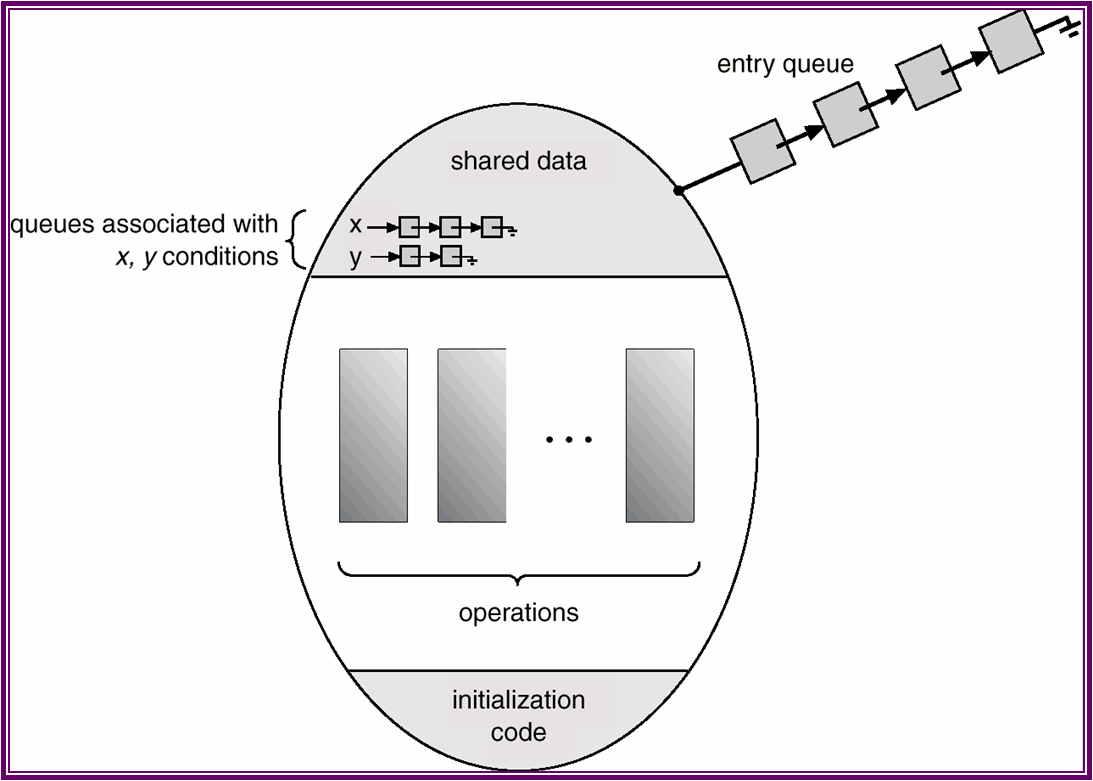
\includegraphics[scale=.5]{v6f7-21}
  \end{center}
  \end{frame}

  %% PAGE
  \begin{frame}
  \frametitle{What happens after a \emph{c.signal()}?} \pause
  \begin{itemize}
  \item{Suppose a process \emph{P} is invoking \emph{c.signal()} and another
    process \emph{Q} is blocked by the condition variable \emph{c}.} \pause
  \item{After \emph{P} completed the \emph{c.signal()}, it's possible that
    both \emph{P} and \emph{Q} will be active simultaneously within the monitor.} \pause
    \begin{itemize}
    \item{This will break the property of the monitor!} \pause
    \end{itemize}
  \item{Three possibilities exist:} \pause
    \begin{itemize}
    \item{Hoare-style: suspending \emph{P} and letting \emph{Q} run.} \pause
    \item{Brinch-Hansen-style: \emph{P} must leave the monitor immediately.} \pause
    \item{Mesa-style (Mesa is a programming language): letting \emph{P} run and suspending \emph{Q}.}
    \end{itemize}
  \end{itemize}
  \end{frame}

  \subsection{Monitor solution to the dining-philosopher problem}

  %% PAGE
  \begin{frame}[fragile]
  \frametitle{Monitor solution to the dining-philosopher problem} \pause

\begin{lstlisting}
monitor dp {
  enum {THINKING, HUNGRY, EATING} state[N];
  condition c[N];
\end{lstlisting}

  \begin{minipage}[c]{0.5\textwidth}
\begin{lstlisting}
  void take_forks(int i) {
    state[i] = HUNGRY;
    test(i);
    if(state[i] != EATING)
      c[i].wait();
  }
\end{lstlisting}

  \end{minipage}%
  \begin{minipage}[c]{0.5\textwidth}

\begin{lstlisting}
  void put_forks(int i) {
    state[i] = THINKING;
    test(LEFT);
    test(RIGHT);
  }
\end{lstlisting}
  \end{minipage}

\begin{lstlisting}
  void test(int i) {
    if(state[i] == HUNGRY &&
       state[LEFT] != EATING &&
       state[RIGHT] != EATING) {
      state[i] = EATING;
      c[i].signal();
    }
  }
  void init() {
    for(int i = 0; i < N; i++)
      state[i] = THINKING;
  }
}
\end{lstlisting}

\end{frame}

  %% PAGE
  \begin{frame}
  \frametitle{Questions}
  \begin{itemize}
  \item{Any questions?}
  \end{itemize}
  \begin{center}
    
\includegraphics[scale=.5]{question}
  \end{center}
  \end{frame}

  \subsection{Language support}

  %% PAGE
  \begin{frame}
 \frametitle{Language support} \pause
 \begin{itemize}
 \item{The monitor constructs must be supported by the programming language to be useful.} \pause
   \begin{itemize}
   \item{That is, the compiler must recognize the monitor construct and
     generate codes to support its functionality.} \pause
   \end{itemize}
 \item{Example: Java (Mesa-style monitor with only one condition variable)} \pause
     \begin{itemize}
     \item{By adding the keyword \emph{synchronized} to a method declaration,
       Java guarantees that once any thread has started executing that method,
       no other thread will be allowed to start executing any other \emph{synchronized} method in that class.} \pause
     \item{And Java provides two operations: \emph{wait} and \emph{notify} to block and wakeup the thread.}
     \end{itemize}
 \end{itemize}
  \end{frame}

\iffalse

  %% PAGE
  \begin{frame}
  \frametitle{Language support (2/2)} \pause
% \begin{itemize}\parskip=0pt
% \item{Examples} \pause  % FIXME
   \begin{itemize}\parskip=0pt
   \item{OpenMP (supports critical-region, www.openmp.org)} \pause
     \begin{itemize}\parskip=0pt
     \item{A specification for a set of compiler directives, library routines,
       and environment variables that can be used to specify shared-memory parallelism in Fortran and C/C++ programs.} \pause
     \item{Compilers supporting OpenMP} \pause
       \begin{itemize}\parskip=0pt
       \item{Intel C/C++ Compiler, Microsoft Visual Studio 2005, GCC} \pause
       \end{itemize}
     \end{itemize}
   \item{Java (supports Mesa-style monitor with only one condition variable)} \pause
     \begin{itemize}\parskip=0pt
     \item{By adding the keyword \emph{synchronized} to a method declaration,
       Java guarantees that once any thread has started executing that method,
       no other thread will be allowed to start executing any other \emph{synchronized} method in that class.} \pause
     \item{And Java provides two operations: \emph{wait} and \emph{notify} to block and wakeup the thread.}
     \end{itemize}
   \end{itemize}
% \end{itemize}
  \end{frame}

\fi

  %% PAGE
  \begin{frame}
  \frametitle{Questions}
  \begin{itemize}
  \item{Any questions?}
  \end{itemize}
  \begin{center}
    
\includegraphics[scale=.5]{question}
  \end{center}
  \end{frame}

\section{Relationships of semaphore and monitor}

\iffalse

  %% PAGE
  \begin{frame}
  \frametitle{Relationship of various synchronization constructs (1/2)} \pause
  \begin{itemize}
  \item{Synchronization constructs introduced so far is \emph{equivalent} in their functionality.} \pause
    \begin{itemize}
    \item{The critical-region can be implemented using semaphore and vice verse.} \pause
    \item{The monitor can be implemented using semaphore and vice verse.} \pause
    \item{The critical-region can be implemented using monitor and vice verse.}
    \end{itemize}
  \end{itemize}
  \end{frame}

\fi

  %% PAGE
  \begin{frame}
  \frametitle{Relationship of semaphore and monitor} \pause
  \begin{itemize}
  \item{Semaphore and monitor are \emph{equivalent} in their functionality.} \pause
    \begin{itemize}
    \item{But their use and implementation are quite different.} \pause
    \end{itemize}
  \end{itemize}
  \begin{center}
    \includegraphics[scale=.5]{psr}
  \end{center}
  \end{frame}

\iffalse

  %% PAGE
  \begin{frame}[fragile]
  \frametitle{Implement semaphore using critical-region} \pause

\begin{lstlisting}
                        struct {
                          int value;
                        } semaphore;
\end{lstlisting} \pause
  \begin{minipage}[c]{0.5\textwidth}

\begin{lstlisting}
  P(semaphore s) {
    region s when (value > 0) {
      value--;
    }
  }
\end{lstlisting}

  \pause

\end{minipage}%
\begin{minipage}[c]{0.5\textwidth}

\begin{lstlisting}
V(semaphore s) {
  region s when (true) {
    value++;
  }
}
\end{lstlisting}

    \end{minipage}

\end{frame}

  %% PAGE
  \begin{frame}[fragile]
  \frametitle{Implement critical-region using semaphore} \pause

\begin{lstlisting}
 // region v when B do S;
 semaphore mutex, first_delay, second_delay;
 int first_count, second_count;
\end{lstlisting}
  \pause
  \begin{minipage}[c]{0.4\textwidth}

\begin{lstlisting}
P(&mutex);
while(!B) {
  first_count++;
  if(second_count > 0)
    V(&second_delay);
  else
    V(&mutex);
  P(&first_delay);
  first_count--;
  second_count++;
  if(first_count > 0)
    V(&first_delay);
  else
    V(&second_delay);
  P(&second_delay);
  second_count--;
 }
\end{lstlisting} \pause

  \end{minipage}%
  \begin{minipage}[c]{0.2\textwidth}

\begin{lstlisting}
S;
\end{lstlisting}

    \pause
  \end{minipage}%
  \begin{minipage}[c]{0.4\textwidth}

\begin{lstlisting}
 if(first_count > 0)
   V(&first_delay);
 else if (second_count > 0)
   V(&second_delay);
 else
   V(&mutex);
\end{lstlisting}

  \end{minipage}
\end{frame}

\fi

  %% PAGE
  \begin{frame}[fragile]
  \frametitle{Implement semaphore using monitor} \pause

\begin{lstlisting}
                        monitor semaphore {
                          int value;
                          condition c;

                          void P() {
                            value--;
                            if(value < 0)
                              c.wait();
                          }

                          void V() {
                            value++;
                            if(value <= 0)
                              c.signal();
                          }
                        }
\end{lstlisting}

\end{frame}

  %% PAGE
  \begin{frame}[fragile]
  \frametitle{Implement monitor using semaphore} \pause

\begin{lstlisting}
                        semaphore mutex = 1, next = 0;
                        int next_count = 0;

                        // for each condition variable x
                        semaphore x_sem = 1;
                        int x_count = 0;
\end{lstlisting} \pause

  \begin{minipage}[c]{0.4\textwidth}

\begin{lstlisting}
// Mutual exclusion
// within a monitor
P(&mutex);
...
body of F;
...
if(next_count > 0)
  V(&next);
else
  V(&mutex);
\end{lstlisting}
    \pause

  \end{minipage}%
  \begin{minipage}[c]{0.3\textwidth}

\begin{lstlisting}
// x.wait()
x_count++;
if(next_count > 0)
  V(&next);
else
  V(&mutex);
P(&x_sem);
x_count--;
\end{lstlisting}

    \pause

  \end{minipage}%
  \begin{minipage}[c]{0.3\textwidth}
\begin{lstlisting}
// x.signal()
if(x_count > 0) {
  next_count++;
  V(&x_sem);
  P(&next);
  next_count--;
}
\end{lstlisting}

  \end{minipage}
\end{frame}

  %% PAGE
  \begin{frame}
  \frametitle{Questions}
  \begin{itemize}
  \item{Any questions?}
  \end{itemize}
  \begin{center}
    
\includegraphics[scale=.5]{question}
  \end{center}
  \end{frame}

\end{CJK*}
\end{document}
